\documentclass[12pt,a4paper]{article}
\usepackage[a4paper, left=3.5cm, right=2cm, top=2.5cm, bottom=3cm,footskip=.25in]{geometry}
\usepackage[utf8]{inputenc}
\usepackage[T1]{fontenc}
\usepackage{amsmath}
\usepackage{amssymb}
\usepackage{lmodern}
\usepackage{indentfirst}
\usepackage{enumerate}
\usepackage{array}
\usepackage{float}
\usepackage{ragged2e}
\usepackage{lipsum}
\usepackage{titlesec}
\usepackage[pdftex]{graphicx}
\graphicspath{{.png}{images/}}
\renewcommand{\baselinestretch}{1.8}

\usepackage{pdfpages}

\usepackage{hyperref}
\hypersetup{colorlinks=true, linkcolor=black}

\titlespacing*{\section}
{0pt}{5.5ex plus 1ex minus .2ex}{4.3ex plus .2ex}
\titlespacing*{\subsection}
{0pt}{5.5ex plus 1ex minus .2ex}{4.3ex plus .2ex}

\usepackage{soul}
\newcommand{\ol}[1]{{\setul{-1.2em}{}\ul{#1}}}
\newcommand{\textoverline}[1]{{\setul{-5em}{}$\overline{\mbox{#1}}$}}

\newtheorem{definition}{Definition}[subsection]
\newtheorem{example}{Example}[subsection]

\usepackage[round]{natbib}
\usepackage{tikz-qtree}
\usepackage{tikz}
\usetikzlibrary{arrows}
\usetikzlibrary{decorations.text}

\usepackage{pifont}
\newcommand{\xmark}{\ding{53}}

\begin{document}

\begin{titlepage}
	\centering
	\par\vspace{1cm}
	{\scshape\bf FACULTY OF MATHEMATICS, PHYSICS AND INFORMATICS \par}
	{\scshape\bf OF THE COMENIUS UNIVERSITY IN BRATISLAVA \par}
	\par\vspace{8cm}
	{\scshape\bf OPTIMIZATION OF AN ABDUCTIVE REASONER FOR DESCRIPTION LOGICS \par}
	\par\vspace{0.5cm}
	{\textsc Master thesis \par}
	\par\vspace{10.6cm}
	{\scshape\bf 2019 \hfill Katarína Fabianová \par}
\end{titlepage}

\pagebreak
\thispagestyle{empty}
\centering
\par\vspace{1cm}
{\scshape\bf FACULTY OF MATHEMATICS, PHYSICS AND INFORMATICS \par}
{\scshape\bf OF THE COMENIUS UNIVERSITY IN BRATISLAVA \par}
\par\vspace{8cm}
{\scshape\bf OPTIMIZATION OF AN ABDUCTIVE REASONER FOR DESCRIPTION LOGICS \par}
\par\vspace{0.5cm}
{\textsc Master thesis \par}
\par\vspace{2cm}
\begin{table*}[ht]
	\newcolumntype{x}[1]{>{\hspace{0pt}}p{#1}}
	\begin{tabular}{@{}x{5cm}x{10cm}@{}}
		Study program: & Applied informatics \\
		Field of study: & 2511 Applied informatics \\
		School department: & Department of Applied Informatics \\
		Adviser: & Mgr. Júlia Pukancová, PhD. \\
		Consultant: & RNDr. Martin Homola, PhD. \\
	\end{tabular}
\end{table*}
\par\vspace{3.03cm}
{\scshape\bf Bratislava 2019 \hfill Katarína Fabianová \par}

\pagebreak

\justify

%\pagebreak
%\thispagestyle{empty}
%\par\vspace*{15cm}
%{\large\bf Dedication \par}
%\par\vspace{0.8cm}
%\large Čestne prehlasujem, že prácu som vypracovala samostatne
%pod vedením školiteľa a uviedla som všetky použité
%zdroje informácií a použitú literatúru. \par
%\par\vspace{3cm}
%\large {Bratislava \hfill \textoverline{Katarína Fabianová}} \par

\pagebreak
\thispagestyle{empty}
\par\vspace*{15cm}
{\large\bf Acknowledgements \newline \par}

\pagebreak
\thispagestyle{empty}
{\large\bf Abstract \newline \par} 

\textbf{Key words:}

\pagebreak
\thispagestyle{empty}
{\large\bf Abstrakt \newline \par} 

\textbf{Kľúčové slová:}

\pagebreak
\thispagestyle{empty}
\tableofcontents
\thispagestyle{empty}

\pagebreak
\thispagestyle{empty}
\listoffigures

\pagebreak
\section*{Introduction}
\addcontentsline{toc}{section}{\protect\numberline{}Introduction}


\pagebreak
\section{Description logics}
Description logics (DLs) are a family of knowledge representation formalism. Each description logic has different expressivity. Every expressivity is expressed with a unique set of constructors. We are going to work with $\mathcal{ALC}$, $\mathcal{EL}$ and $\mathcal{EL}${+}{+} DL. Each description logic has its own syntax and semantics. In this chapter we will introduce syntax and semantics \citep{Rudolph2011} for each DL that we will be working with.

\subsection{$\mathcal{ALC}$ DL}
$\mathcal{ALC}$ DL is a DL which is more expressive than $\mathcal{EL}$ and $\mathcal{EL}{+}{+}$ DL. $\mathcal{ALC}$ is less expressive than many other DLs. $\mathcal{ALC}$ stands for Attributive (Concept) Language with Complements. It means that not only complement of atomic concept is allowed but also a complement of complex concept is allowed.

\subsubsection{$\mathcal{ALC}$ Syntax}
$\mathcal{ALC}$ description logic consists of three mutually disjoint sets. These sets represent whole vocabulary that is used by $\mathcal{ALC}$ DL.

\begin{definition}{\textbf{DL vocabulary}}
	\[ \textbf{Set of individuals:} \text{ } N_{I} = \{a,b,c...\} \]
	\[ \textbf{Set of concepts:} \text{ } N_{C} = \{A,B,C...\} \]
	\[ \textbf{Set of roles:} \text{ } N_{R} = \{R_{1},R_{2},R_{3},...\} \]
\end{definition}

\begin{example}{\textbf{DL vocabulary}}
	\[ N_{I} = \{ jack, john, jane \} \]
	\[ N_{C} = \{ Person, Mother, Father \} \]
	\[ N_{R} = \{ hasChild, likes, owns \} \]
\end{example}

$\mathcal{ALC}$ DL deals with individuals and concepts. An individual is a concrete instance of a concept. Concept is a class that defines some entity. Concept can be atomic or complex. Atomic concept is not constructed with any constructor. On the contrary complex concept is created from constructors and other concepts.

\begin{definition}{\textbf{Complex concept}}
	
	Concepts are recursively constructed as the smallest set of expressions of the forms:
	\[ C,D ::= A | \neg C | C \sqcap D | C \sqcup D | \exists R.C | \forall R.C \]
	where $A \in N_{C}$, $R \in N_{R}$, and C, D are concepts.
\end{definition}

\begin{example}{\textbf{Complex concept}}
\[ \neg Mother \]
\[ Mother \sqcup Father \]
\[ \exists hasChild.Person \]
\[ \forall likes.Food \]
\end{example}

Complex concept uses following constructors: $\neg$, $\sqcup$, $\sqcap$, $\exists$ and $\forall$. Constructor $\neg$ is negation, constructor $\sqcup$ is or and constructor $\sqcap$ is and. Constructors $\exists$ is existential restriction and $\forall$ is called value restriction.

There are two concepts that are always in ontology. $\top$ (top) stays for everything. Each concept belongs under $\top$ which means that each concept is on left side of subsumption if on right side is only $\top$. Second concept is $\bot$ (bottom) and it stays for nothing which means that each concept is on the right side of subsumption if there is only $\bot$ on the left side. Formally these two concepts can be written as follows:
\[ \top \equiv A \sqcup \neg A \]
\[ \bot \equiv A \sqcap \neg A \]

$\mathcal{ALC}$ description logic uses axioms in order to model some situation. Ontology \citep{staabHandbookOntology} is used to formally describe these axioms. The purpose of ontology is to describe relationships between entities in a formal language. Every ontology has its own knowledge base. Knowledge base is a set of TBox axioms and ABox axioms. Ontology is described by knowledge base.

\begin{definition}{\textbf{Knowledge base}}
	
	Knowledge base ($\mathcal{KB}$) is an ordered pair of \textit{TBox} $\mathcal{T}$ and \textit{ABox} $\mathcal{A}$.
\end{definition}

\begin{example}{\textbf{Knowledge base}}
	\[ 
	\mathcal{KB} = \left\{
	\begin{tabular}{c c}
	$Professor \sqcup Scientist \sqsubseteq Academician$ \\
	$AssocProfessor \sqsubseteq Professor$ \\
	$jack : Academician$ \\
	$jane : Scientist$ \\
	$john : Professor$ \\	
	\end{tabular}
	\right \}
	\]
\end{example}

There are two types of axioms, the first is TBox and the second one is ABox. In TBox the subsumption symbol ($\sqsubseteq$) is used. Let's explain this symbol on an example $Mother \sqsubseteq Parent$. $Mother$ is always a $Parent$ but $Parent$ does not always have to be a $Mother$. TBox represents axioms that model ontology. Each axiom explains the relationship between entities in this axiom.

\begin{definition}{\textbf{TBox}}
	
	A TBox $\mathcal{T}$ is a finite set of GCI axioms $\phi$ of the form:
	\[ \phi ::= C \sqsubseteq D \]	
	where C, D are any concepts.
\end{definition}

\begin{example}{\textbf{TBox}}
	\[ 
	\mathcal{T} = \left\{
	\begin{tabular}{c c}
	$Professor \sqcup Scientist \sqsubseteq Academician$ \\
	$AssocProfessor \sqsubseteq Professor$ \\
	\end{tabular}
	\right \}
	\]
\end{example}

ABox on the other side does not model ontology but creates a database of facts. It contains set of assertion axioms that can be called facts. Fact is a direct assertion of an individual to a concept.

\begin{definition}{\textbf{ABox}}
	
    An ABox $\mathcal{A}$ is a finite set of assertion axioms $\phi$ of the form:
	\[ \phi ::= a:C | a,b:R \]
	where $a,b \in N_{I}$, $R \in N_{R}$ and C is any concept.
\end{definition}

\begin{example}{\textbf{ABox}}
	\[ 
	\mathcal{A} = \left\{
	\begin{tabular}{c c}
	$jack : Academician$ \\
	$jane : Scientist$ \\
	$john : Professor$ \\
	\end{tabular}
	\right \}
	\]
\end{example}

To have a better understanding of $\mathcal{ALC}$ DL we can translate sentences into $\mathcal{ALC}$ description logic.

\[ \text{Everybody who is sick, is not happy.} \]
\[ Sick \sqsubseteq \neg Happy \]

\[ \text{Cat and dogs are animals.} \]
\[ Cat \sqcup Dog \sqsubseteq Animal \]

\[ \text{Every person owns a house.} \]
\[ Person \sqsubseteq \exists owns.House \]

\subsubsection{$\mathcal{ALC}$ Semantics}
An interpretation is a pair of a domain and an interpretation function. The domain is a set of values that represents concepts in the interpretation. The result of interpretation function is different for individuals, concepts and roles. If we use the interpretation function on an individual the result is an element from the domain. If we use it on the concepts the result is a set of elements from the domain. If we use it on the roles the result is a set of pairs of elements from the domain.

\begin{definition}{\textbf{Interpretation}}

	An interpretation of a given knowledge base $\mathcal{KB} = (\mathcal{T}, \mathcal{A})$ is a pair $\mathcal{I} = (\Delta^{\mathcal{I}}, \cdot ^{\mathcal{I}})$ which contains a domain $\Delta^{\mathcal{I}}$ and an interpretation function $\cdot ^{\mathcal{I}}$.	
	Domain can not be empty.
		
	The interpretation function is following:
	\[ a^{\mathcal{I}} \in \Delta^{\mathcal{I}} \text{ } \forall a \in N_{I} \]
	\[ A^{\mathcal{I}} \subseteq \Delta^{\mathcal{I}} \text{ } \forall A \in N_{C} \]
	\[ R^{\mathcal{I}} \subseteq \Delta^{\mathcal{I}} \times \Delta^{\mathcal{I}} \text{ } \forall R \in N_{R} \]
	The interpretation of complex concepts is recursively defined:
	\[ \neg C^{\mathcal{I}} = \Delta^{\mathcal{I}} \backslash C^{\mathcal{I}} \]
	\[ C \sqcap D^{\mathcal{I}} = C^{\mathcal{I}} \cap D^{\mathcal{I}} \]
	\[ C \sqcup D^{\mathcal{I}} = C^{\mathcal{I}} \cup D^{\mathcal{I}} \]
	\[ \exists R.C^{\mathcal{I}} = \{ x \in \Delta^{\mathcal{I}} | \exists y \in \Delta^{\mathcal{I}} : \langle x,y \rangle \in R^{\mathcal{I}} \land y \in C^{\mathcal{I}} \} \]
	\[ \forall R.C^{\mathcal{I}} = \{ x \in \Delta^{\mathcal{I}} | \forall y \in \Delta^{\mathcal{I}} : \langle x,y \rangle \in R^{\mathcal{I}} \rightarrow y \in C^{\mathcal{I}} \} \]
\end{definition}

\begin{example}{\textbf{Interpretation}}
	\[ 
	\mathcal{KB} = \left\{
	\begin{tabular}{c c}
	$Professor \sqcup Scientist \sqsubseteq Academician$ \\
	$AssocProfessor \sqsubseteq Professor$ \\
	$jack : Academician$ \\
	\end{tabular}
	\right \}
	\]
	
	\[ \mathcal{I} = (\Delta ^{\mathcal{I}}, \cdot^{\mathcal{I}}) \]
	\[ \Delta ^{\mathcal{I}} = \{ P,S,A,AP \} \]
	\[ Professor^{\mathcal{I}} = \{P\} \]
	\[ Scientist^{\mathcal{I}} = \{S\} \]
	\[ Academician^{\mathcal{I}} = \{A\} \]
	\[ AssocProfessor^{\mathcal{I}} = \{AP\} \]
	\[ jack^{\mathcal{I}} = A \]
	
\end{example}

The interpretation satisfies an axiom according to its type. We know three types of axioms. The first is an axiom from TBox, the second one is an assertion axiom to a concept and the third one is an assertion to a role.

\begin{definition}{\textbf{Satisfaction $\models$}}

	Given an axiom $\phi$, an interpretation $\mathcal{I} = (\Delta^{\mathcal{I}}, \cdot ^{\mathcal{I}})$ satisfies $\phi (\mathcal{I} \models \phi)$ depending on its type:
	\[ \mathcal{I} \models C \sqsubseteq D \text{ iff } C^{\mathcal{I}} \subseteq D^{\mathcal{I}} \]
	\[ \mathcal{I} \models a:C \text{ iff } a^{\mathcal{I}} \in C^{\mathcal{I}} \]
	\[ \mathcal{I} \models a,b:R \text{ iff } \langle a^{\mathcal{I}}, \in b^{\mathcal{I}} \rangle \in R^{\mathcal{I}} \]	
\end{definition}

Finding a model (an interpretation satisfying $\mathcal{KB}$) is crucial for consistency checking. If we find at least one model the knowledge base $\mathcal{KB}$ is consistent. We can have more models for one knowledge base. In Example 1.1.7 there are two showed models but there can be more models. 

\begin{definition}{\textbf{Model}}
	
	An interpretation $\mathcal{I} = \langle \Delta^{\mathcal{I}}, \cdot ^{\mathcal{I}}  \rangle$ is a model of a DL knowledge base $\mathcal{KB} = (\mathcal{T}, \mathcal{A})$ iff $\mathcal{I}$ satisfies every axiom in TBox $\mathcal{T}$ and ABox $\mathcal{A}$.
\end{definition}

\begin{example}{\textbf{Model}}
	\[ 
	\mathcal{KB} = \left\{
	\begin{tabular}{c c}
	$Professor \sqcup Scientist \sqsubseteq Academician$ \\
	$AssocProfessor \sqsubseteq Professor$ \\
	$jack : Academician$ \\
	\end{tabular}
	\right \}
	\]

	\[ \mathcal{I}_{1} = \{  \Delta^{\mathcal{I}} = \{ P,S,A,AP \}, \]	
	\[ Professor^{\mathcal{I}} = \{P\}, Scientist^{\mathcal{I}} = \{S\}, Academician^{\mathcal{I}} = \{A\}, AssocProfessor^{\mathcal{I}} = \{AP\} \]
	\[ jack^{\mathcal{I}} = A \} \]	

	\[ \mathcal{I}_{2} = \{  \Delta^{\mathcal{I}} = \{ A \}, \]	
	\[ Professor^{\mathcal{I}} = \{A\}, Scientist^{\mathcal{I}} = \{A\}, Academician^{\mathcal{I}} = \{A\}, AssocProfessor^{\mathcal{I}} = \{A\} \]
	\[ jack^{\mathcal{I}} = A \} \]		
\end{example}

\begin{definition}{\textbf{Consistency}}
	
	A knowledge base $\mathcal{KB}$ is consistent iff $\mathcal{KB}$ has at least one model $\mathcal{I}$.
\end{definition}

We are familiar with more decision problems, satisfiability, subsumption $(\sqsubseteq)$, equivalence ($\equiv$) and disjointness. Satisfiability means that concept is satisfiable in regard to $\mathcal{KB}$ if we can find such a model of a knowledge base for which holds that interpretation of that concept is not empty. Subsumption between two concepts must hold that interpretation of left-sided concept is a proper subset of interpretation of right-sided concept in each possible model of a knowledge base. Equivalence is similar to subsumption but the difference is that the interpretations of both concepts must be equal in each possible model of a knowledge base. Disjointness means that intersection of the interpretations of both concepts must be an empty set in each possible model of a knowledge base.

\begin{definition}{\textbf{Decision problems}}

	Given a DL $\mathcal{KB} = (\mathcal{T}, \mathcal{A})$, and two concepts C,D, we say that:

	\begin{itemize}
		\item $C \text{ is satisfiable w.r.t. } \mathcal{KB} \text{ iff there is such a model } \mathcal{I} \text{ of } \mathcal{KB} \text{ for which holds that } \newline C^{\mathcal{I}} \neq \emptyset;$

		\item $C \text{ is subsumed by D w.r.t. } \mathcal{KB} \text{ (denoted } \mathcal{KB} \models C \sqsubseteq D) \text{ iff } C^{\mathcal{I}} \subseteq D^{\mathcal{I}} \text{ in every} \newline \text{model } \mathcal{I} \text{ of } \mathcal{KB};$

		\item $\text{C and D are equivalent w.r.t. } \mathcal{KB} \text{ (denoted } \mathcal{KB} \models C \equiv D) \text{ iff } C^{\mathcal{I}} = D^{\mathcal{I}} \text{ in every} \newline \text{model } \mathcal{I} \text{ of } \mathcal{KB};$
		
		\item $\text{C and D are disjoint w.r.t. } \mathcal{KB} \text{ iff } C^{\mathcal{I}} \cap D^{\mathcal{I}} = \emptyset \text{ in every model } \mathcal{I} \text{ of } \mathcal{KB}.$		
	\end{itemize}
\end{definition}

If $\mathcal{KB} = \emptyset$ then we say that decision problems (satisfiability, subsumption, equivalence and disjointness) of concepts are defined in general by definition and we use notation such as we omit $\mathcal{KB} \models$ from the notation.

\subsection{DL Tableau algorithm}
Following definitions \citep{baaderHandbook} describe rules and terms that are used by this algorithm. DL Tableau algorithm proves satisfiability of a concept or checks consistency of a given knowledge base. By proving satisfiability the input for the algorithm is concept C and TBox $\mathcal{T}$. By checking consistency the input for the algorithm is a knowledge base $\mathcal{KB}$. In both versions of this algorithm holds that each concept must be in NNF (negation normal form). Negation normal form is such a form that each negation is pushed in front of atomic concept inside a complex concept. 

\begin{definition}{\textbf{NNF}}
	
	A concept C is in NNF (negation normal form) iff the complement constructor $\neg$ 
	only occurs in front of atomic concept symbols inside C.
\end{definition}

\begin{example}{\textbf{NNF}}
	\[ nnf(\neg (C \sqcap D)) = \neg C \sqcup \neg D \]
	\[ nnf(\neg (C \sqcup D)) = \neg C \sqcap \neg D \]
	\[ nnf(\neg \exists R.C) = \forall R. \neg C \]
	\[ nnf(\neg \forall R.C) = \exists R. \neg C \]
\end{example}

DL Tableau algorithm creates a CTree (Completion tree). CTree proves whether model exists or not.

\begin{definition}{\textbf{Completion tree}}

	A completion tree (CTree) is a triple T = (V, E, $\mathcal{L}$) where (V, E)
	is a tree and $\mathcal{L}$ is a labeling function which means that:
	$\mathcal{L}(x)$ is a set of concepts $\forall x \in V$ and
	$\mathcal{L}(\langle x, y \rangle )$ is a set of roles $\forall \langle x, y \rangle \in E$.	
\end{definition}

At first the algorithm creates node and initializes it with the input concept.
Then the algorithm applies tableau rules for given DL. If the algorithm applies each rule until any rule can be applied and it finds no clash then result is that concept C is satisfiable w.r.t. $\mathcal{T}$.

\begin{definition}{\textbf{Successor, R-successor}}

	Given a CTree T = (V,E, $\mathcal{L}$) and $x,y \in V$ we say that: 
	\begin{itemize}
		\item y is a successor of x iff $\langle x,y \rangle \in E$
		\item y is an R-successor of x iff $\langle x,y \rangle \in E$ and $R \in \mathcal{L}(\langle x,y \rangle)$.
	\end{itemize}
\end{definition}

\begin{definition}{\textbf{Clash}}

	There is a clash in a CTree T = $(V,E, \mathcal{L})$ if and only iff for some $x \in V$ and for some concept C both $C \in \mathcal{L}(x)$ and $\neg C \in \mathcal{L}(x)$.
\end{definition}

\begin{example}{\textbf{Clash}}
	\[ \mathcal{L}(s_{0}) = \{ C, D, \neg D \} \]
\end{example}

\begin{definition}{\textbf{Clash-free CTree}}

A CTree T = $(V,E, \mathcal{L})$ is clash-free iff none of the nodes in V contains a clash.
\end{definition}

There can be a situation that some concept can lead to infinite looping and algorithm would never stop. An example for that is: $Person \sqsubseteq \exists hasParent.Person$. That is why the algorithm uses Blocking rule.

\begin{definition}{\textbf{Blocking}}
	
	Given a CTree $T = (V, E, \mathcal{L})$ a node $x \in V$ is blocked if it has an ancestor $y$ such that: either $\mathcal{L}(x) \subseteq \mathcal{L}(y)$ or $y$ is blocked.
\end{definition}

DL Tableau algorithm proves concept satisfiability in regard of TBox. Input for DL Tableau algorithm is concept C and TBox $\mathcal{T}$. Output is a boolean value which is true if concept C is satisfiable w.r.t. $\mathcal{T}$, false otherwise.

\begin{definition}{\textbf{Algorithm - Concept satisfiability}}	
	
	\noindent \textbf{Input:} concept C and $\mathcal{T}$ in NNF \newline
	\textbf{Output:} answers whether concept C is satisfiable w.r.t. $\mathcal{T}$ or not \newline
	\textbf{Steps:}
	\begin{enumerate}
		\item Initialize a new CTree T := $(\{s_{0}\}, \emptyset, \{s_{0} \rightarrow \{C\}\})$;
		\item Apply tableau rules for TBoxes while at least one rule is applicable;
		\item Answer "C is satisfiable w.r.t. $\mathcal{T}$" if T is clash-free. Otherwise answer "C is unsatisfiable w.r.t. $\mathcal{T}$".
	\end{enumerate}
\end{definition}	

\begin{definition}{\textbf{$\mathcal{ALC}$ tableau rules for TBoxes}}
	\begin{itemize}
		\item $\sqcap-rule:$ if $C_{1} \sqcap C_{2} \in \mathcal{L}(x)$ and $x \in V$ and $\{ C_{1}, C_{2} \} \not \subseteq \mathcal{L}(x)$ and x is not blocked then $\mathcal{L}(x) = \mathcal{L}(x) \cup \{ C_{1}, C_{2} \}$
		
		\item $\sqcup-rule:$ if $C_{1} \sqcup C_{2} \in \mathcal{L}(x)$ and $x \in V$ and $ \{ C_{1}, C_{2} \} \cap \mathcal{L}(x) = \emptyset$ and x is not blocked then either $\mathcal{L}(x) = \mathcal{L}(x) \cup \{ C_{1} \}$ or $\mathcal{L}(x) = \mathcal{L}(x) \cup \{ C_{2} \}$
		
		\item $\forall-rule:$ if $\forall R.C \in \mathcal{L}(x)$ and $x,y \in V$ and y is R-successor of x and $C \not \in \mathcal{L}(y)$ and x is not blocked then $\mathcal{L}(y) = \mathcal{L}(y) \cup \{ C \}$
		
		\item $\exists-rule:$ if $\exists R.C \in \mathcal{L}(x)$ and $x \in V$ with no R-successor y and $C \in \mathcal{L}(y)$ and x is not blocked then $\mathcal{V} = \mathcal{V} \cup \{ z \}, \mathcal{L}(z) = \{ C\}$ and $\mathcal{L}( \langle x, z \rangle ) = \{ R \}$
		
		\item $\mathcal{T}-rule:$ if $C_{1} \sqsubseteq C_{2} \in \mathcal{T}$ and $x \in V$ and nnf$(\neg C_{1} \sqcup C_{2}) \not \in \mathcal{L}(x)$ and x is not blocked then $\mathcal{L}(x) = \mathcal{L}(x) \cup \{ nnf(\neg C_{1} \sqcup C_{2}) \}$
	\end{itemize}
\end{definition}	

Knowledge base is a pair of a TBox and an Abox and yet only a TBox was mentioned in connection with the DL Tableau algorithm. If we also have a given ABox the algorithm must be modified. The algorithm checks no longer concept satisfiability w.r.t. $\mathcal{T}$ but checks consistency of a given $\mathcal{KB}$. The same condition holds for the result as in proving concept satisfiability. If there is a found clash the knowledge base is not consistent otherwise the knowledge base is consistent. Difference between the first version of this algorithm is that here are used named nodes. Name of the node is an instance of a concept that comes from ABox. 

\begin{definition}{\textbf{Algorithm - Consistency checking}}

\noindent \textbf{Input:} $\mathcal{KB} = (\mathcal{T}, \mathcal{A})$ in NNF \newline
\textbf{Output:} answers whether $\mathcal{KB}$ is consistent or not \newline
\textbf{Steps:}
\begin{enumerate}
	\item Initialize a CTree as follows:
		\begin{itemize}
			\item $V := \{ a \text{ } | \text{ individual a occurs in } \mathcal{A} \}$;
			\item $E := \{ \langle a,b \rangle \text{ } | \text{ } a,b : R \in \mathcal{A} \text{ for some role R} \}$;
			\item $\mathcal{L}(a) := \{ nnf(E) \text{ } | \text{ } a:E \in \mathcal{A}\} \text{ for all } a \in V$; \newline
			$\mathcal{L}(\langle a,b \rangle) := \{ R \text{ } | \text{ } a,b:R \in \mathcal{A}\} \text{ for all } \langle a,b \rangle \in E$;
		\end{itemize}
	\item Apply tableau rules for TBoxes while at least one rule is applicable;
	\item Answer "$\mathcal{KB}$ is consistent" if T is clash-free. Otherwise answer "$\mathcal{KB}$ is inconsistent".
\end{enumerate}

\end{definition}

Let's introduce an example where we know a knowledge base $\mathcal{KB}$. DL Tableau algorithm checks if knowledge base is consistent or not.

\begin{example}{(\textbf{DL Tableau algorithm})}
	\[ 
	\mathcal{KB} = \left\{
	\begin{tabular}{c c}
	$Student \sqsubseteq \exists attends.MathCourse$ \\
	$MathCourse \sqsubseteq Course$ \\
	$jack : Student$ \\
	\end{tabular}
	\right \}
	\] \\
\end{example}

\begin{center}
	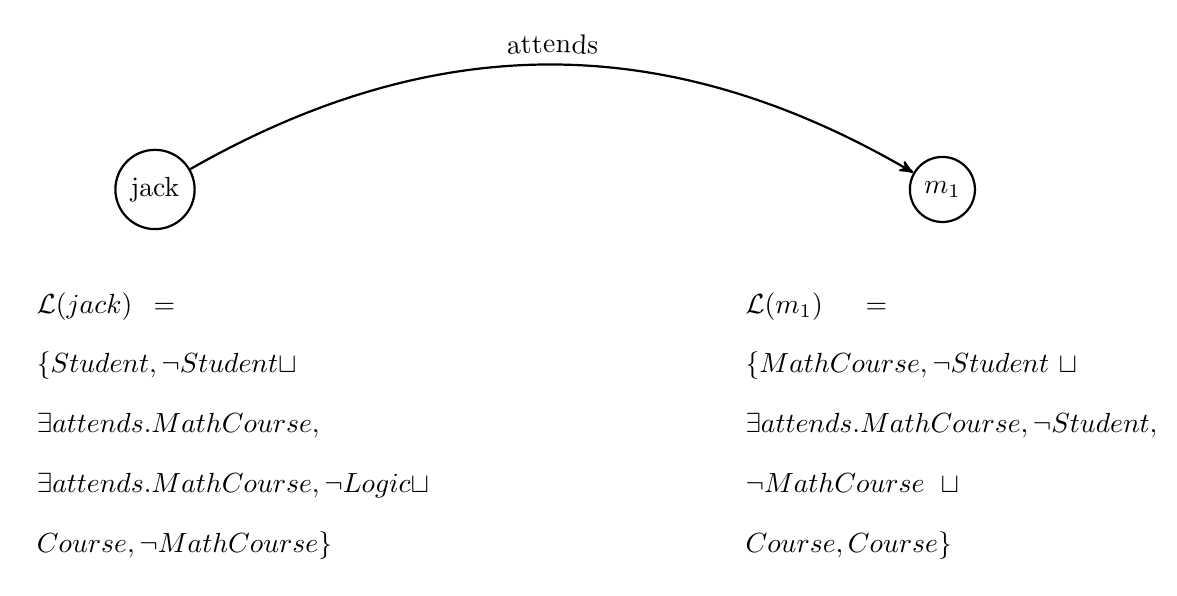
\begin{tikzpicture}[->,>=stealth',auto,node distance=10cm,
	thick,main node/.style={circle, draw}]
	
	\node[main node] (1) {jack};
	\node[main node] (2) [right of=1] {$m_{1}$};
	
	\def\myshift#1{\raisebox{1ex}}
	
	\draw [thick, ->, postaction={decorate, decoration={text along path, text align=center, text={|\myshift|attends}}}] (1) to [bend left=30] (2);
	
	\node[text width=3cm] at (0,-3) 
	{$\mathcal{L}(jack) = \{ Student, \neg Student \sqcup \exists attends.MathCourse, \newline \exists attends.MathCourse, \neg Logic \sqcup Course, \neg MathCourse \}$};		

	\node[text width=5cm] at (10,-3) 
	{$\mathcal{L}(m_{1}) = \{ MathCourse, \neg Student \sqcup \exists attends.MathCourse, \neg Student, \newline \neg MathCourse \sqcup Course, Course \}$};			
	\end{tikzpicture}
\end{center}

The algorithm starts with the ABox assertion axioms. It selects the axiom $jack : Student$. At first it creates a node $jack$ with its label $\mathcal{L}(jack)$. From the assertion axiom $jack : Student$ algorithm knows that jack is a Student and adds the concept $Student$ to the label $\mathcal{L}(jack)$. Then the algorithm is choosing another axiom from the knowledge base. There are no more assertion axioms, so it starts with the axioms from TBox. It takes $Student \sqsubseteq \exists attends.MathCourse$. It must convert it into the negation normal form which is $\neg Student \sqcup \exists attends.MathCourse$. The algorithm applies $\sqcup-rule$. According to this rule it must choose $\exists attends.MathCourse$, otherwise there would be a clash. Now it has to apply $\exists - rule$ so a new node $l_{1}$ will be created with its label $\mathcal{L}(m_{1})$. Concept $MathCourse$ will be added into this label. Let's go back to the $jack$ node. The algorithm has to finish adding all axioms of TBox form. It will add the second axiom from the knowledge base in negation normal form as $\neg MathCourse \sqcup Course$. Now it does not matter which one algorithm chooses if $Course$ or $\neg MathCourse$ because any of these two does not cause a clash. Now the algorithm goes back to the $m_{1}$ node and continues to add axioms from the knowledge base similarly as in the node $jack$. It starts with axiom $\neg Student \sqcup \exists attends.MathCourse$, it will choose the first one $\neg Student$. Then continues with axiom $\neg MathCourse \sqcup Course$. It can not choose $\neg MathCourse$ because there would be immediately a clash. So it chooses $Course$.

The created tree contains two nodes ($jack$ and $m_{1}$) and one edge between them. The edge represents that $jack$ attends some MathCourse $m_{1}$. There is not any instance of a concept $MathCourse$ so the node $m_{1}$ does not represent a concrete instance of the concept $MathCourse$ but represents some instance. There is no clash in both nodes so the answer of the DL Tableau algorithm is that the given knowledge base $\mathcal{KB}$ is consistent.

\section{Abduction}
Generally in logic we are familiar with three ways of thinking. Deduction, induction and abduction. The most known and natural for humans is probably deduction. All three ways are dealing with the following parts: theory, data and effect. In the description logic we can translate the theory as a knowledge base, data as the explanations and the effect as an observation.

By deduction is known a knowledge base and the explanations, the observation is missing and the goal is to deduce the missing observation. By induction is known an observation and an explanation but the knowledge base is unknown. By abduction is known a knowledge base and an observation but the explanation is a subject of searching. All definitions are from article by \cite{pukancovaAboxAbduction}.

\subsection{ABox abduction}
In the description logics abduction is used when we are not familiar with the explanation $\mathcal{E}$ but we know a knowledge base $\mathcal{KB}$ and an observation $\mathcal{O}$. It is important to know that we are looking for minimal explanations. A minimal explanation is such an explanation that it does not exist any other explanation that would be a subset of that minimal explanation.

\begin{definition}{\textbf{(Abduction)}} 

	Given a knowledge base $\mathcal{KB}$ and an observation $\mathcal{O}$, an abductive explanation is such an explanation $\mathcal{E}$ that satisfies $\mathcal{KB} \cup \mathcal{E} \models \mathcal{O}$.
\end{definition}

\begin{definition}{\textbf{(Correct explanation)}}
	\[ \mathcal{E} \text{ is consistent if } \mathcal{E} \cup \mathcal{KB} \not \models \mathcal{\bot}; \] 
	\[ \mathcal{E} \text{ is relevant if } \mathcal{E} \not \models \mathcal{O}; \]
	\[ \mathcal{E} \text{ is explanatory if } \mathcal{KB} \not \models \mathcal{O} \]
\end{definition}

\begin{definition}{\textbf{(Minimal explanation)}}
	
	Minimal explanation is such an explanation that it does not exist any other explanation that would be a subset of this explanation.
\end{definition}

For better understanding of what ABox abduction is let's introduce a few examples. The first example is easy, the searched explanation is obvious but it will demonstrate the problem. The second example is not so obvious that is why we have to use an algorithm to compute the solution. For computing the solution we use the \textbf{Minimal Hitting Set algorithm}.

\begin{example}{(\textbf{ABox Abduction - Emotion})}
	\[ 
	\mathcal{KB} = \left\{
	\begin{tabular}{c c}
	$Sick \sqsubseteq \neg Happy$
	\end{tabular}
	\right \}
	\]
	
	\[ 
	\mathcal{O} = \left\{
	\begin{tabular}{c c}
	$mary : \neg Happy$
	\end{tabular}
	\right \}
	\]								
\end{example}

In this example we are searching the explanations. In this easy assignment it is obvious that what we are looking for is that Mary is sick. If Mary is not happy she must be sick. Formally written solution to this abduction problem is the following:
\[ 
\mathcal{E} = \left\{
\begin{tabular}{c c}
$mary : Sick$
\end{tabular}
\right \}
\]

\begin{example}{(\textbf{ABox Abduction - Academy})}
	\[ 
	\mathcal{KB} = \left\{
	\begin{tabular}{c c}
		$Professor \sqcup Scientist \sqsubseteq Academician$ \\
		$AssocProfessor \sqsubseteq Professor$ \\
	\end{tabular}
	\right \}
	\]
	
	\[ 
	\mathcal{O} = \left\{
	\begin{tabular}{c c}
		$jack : Academician$
	\end{tabular}
	\right \}
	\]								
	
\end{example}

If $jack$ is an Academician he must be a Professor or a Scientist. If he is a Professor he must be also an AssocProfessor. This is an oversimplified explanation how we can retrieve correct explanations. For the better introduction into this algorithm we will explain it step by step. We know the observation so we know that jack is an Academician, that is a fact. In our first axiom in TBox it is written that if somebody is an Academician he is also a Professor or a Scientist. He can be both but at least one of them but that we are not able to determine. That is why both explanations are correct. The second axiom claims that if somebody is a Professor he must be also an AssocProfessor. In this part we are not explaining the whole algorithm yet because it will be explained in our next chapter Minimal Hitting Set algorithm but we need to have at least an idea of how it works. So as we already know the correct explanations are following:

\[ 
\mathcal{E}_{1} = \left\{
\begin{tabular}{c c}
	$jack : Professor$ \\
\end{tabular}
\right \}
\]

\[ 
\mathcal{E}_{3} = \left\{
\begin{tabular}{c c}
	$jack : Scientist$ \\
\end{tabular}
\right \}
\]

\[ 
\mathcal{E}_{3} = \left\{
\begin{tabular}{c c}
	$jack : AssocProfessor$ \\
\end{tabular}
\right \}
\]

\subsection{Minimal Hitting Set algorithm}
In this part we will explain the algorithm: Minimal hitting set. This algorithm is invented by Raymond \cite{reiterHS}. At first we will declare terms that we will be using. The first term is a hitting set. Let's have collection of sets $C$. Hitting set is such a set that has non empty intersection with each set of collection $C$.

\begin{definition}{\textbf{Hitting set}}
	
	A hitting set for a collection of sets $C$ is a set $H \subseteq \cup_{S \in C}$ such that $H \cap S$ is not an empty set for each $S \in C$.
\end{definition}

HS-tree is such a tree that contains nodes with three possible values. The first value is a checkmark, the second is a crossmark and the third is a set. Each edge has its own label that determines path from parent to node. Labeled edges determines path from root to node $n$. HS-tree must be the smallest tree for the collection of sets $C$.

\begin{definition}{\textbf{HS-tree}}
	
	Let $C$ be a collection of sets. An HS-tree $T$ for $C$ is a smallest edge-labeled and node-labeled tree with the following properties:
	
	\begin{itemize}
		\item The root is labeled by $\checkmark$ if $C$ is empty. Otherwise the root is labeled by an arbitrary set of $C$.
		
		\item For each node $n$ of $T$, let $H(n)$ be the set of edge labels on the path in $T$ from the root to a node $n$. The label for $n$ is any set $\sigma \in C$ such that $\Sigma \cap H(n) = \emptyset$, if such a set $\Sigma$ exists. Otherwise, the label for $n$ is $\checkmark$. If $n$ is labeled by the set $\Sigma$, then for each $\sigma \in \Sigma$, $n$ has a successor $n_{\sigma}$ joined to $n$ by an edge of labeled by $\sigma$.
	\end{itemize}
\end{definition}

The Minimal Hitting Set algorithm generates a HS-tree. It is a breadth-first search algorithm which means that algorithm creates all nodes in one breadth level and then it goes to the next level if possible. The following definition describes rules of how the algorithm behaves.

\begin{definition}{\textbf{Minimal Hitting Set algorithm}}{\indent}
	\begin{itemize}
		\item Generate the pruned HS-tree breadth-first, generating all nodes at any fixed level in the tree before descending to generate the nodes at the next level.
		
		\item Reusing node labels: If node $n$ has already been labeled by a set $S \in C$ and if $n'$ is a new node such that $H(n') \cap S = \emptyset$, then label $n'$ by $S$.
		
		\item Tree prunning:
		
		\begin{itemize}
			\item If node $n$ is labeled by $\checkmark$ and node $n'$ is such that $H(n) \subseteq H(n')$, then close the node $n'$. A label is not computed for $n'$ nor are any successor nodes generated.
			
			\item If a node $n$ has been generated and node $n'$ is such that $H(n') = H(n)$, then close node $n'$.
			
			\item If nodes $n$ and $n'$ have been labeled by sets $S$ and $S'$ of $C$, respectively and if $S'$ is a proper subset of $S$, then for each $\alpha \in S - S'$ mark as redundant the edge from node $n$ labeled by $\alpha$. A redundant edge, together with the subtree beneath it, may be removed from the HS-tree while preserving the property that the resulting pruned HS-tree will yield all minimal hitting sets for $C$.
			
		\end{itemize}	
		
	\end{itemize}
	
\end{definition}

Reiter's algorithm is used to compute a minimal hitting set. Input is a set of sets. The goal of Reiter's algorithm is to compute a minimal hitting set from this input. It means that the result hitting set will have non empty intersection with each set from the input.

Let's show an example with $F$ as the input set and $HS$ as the result \label{fig:MinimalHS}.

\begin{example}{\textbf{(Minimal Hitting Set)}}
	\[  F = \{ \{a,b\}, \{b,c\}, \{a,c\}, \{b,d\}, \{b\} \} \]
	\[ HS = \{ \{a,b\}, \{b,c\} \} \]
\end{example}

As we can observe in this example the first result set has non empty intersection with each set of $F$ and the second result set also has intersection with each set of $F$. So we can determine that these result sets are definitely minimal hitting sets. They are both minimal because there is no other set that is smaller and at the same time has non empty intersection with each set of $F$.

For better and easier understanding of this algorithm we can visualize it and explain (Figure \ref*{fig:MinimalHS}).

\begin{figure}[H]
	\centering
	\begin{tikzpicture}[level distance=2.5cm,sibling distance=2cm,
	draw, edge from parent path={(\tikzparentnode) -- (\tikzchildnode)}]
	\Tree
	[.\{a,b\}
		\edge node[auto=right] {a};
		[.\{b,c\} 
			\edge node[midway,left] {b};
			[.{\checkmark} ]
			\edge node[midway,right] {c};
			[.\{b,d\} 
				\edge node[midway,left] {b};
				[.{\xmark} ]
				\edge node[midway,right] {d};
				[.\{b\} 
					\edge node[midway,right] {b};
					[.{\xmark} ]
				]
			]			
		]
		\edge node[auto=left] {b};
		[.\{a,c\} 
			\edge node[midway,left] {a};
			[.{\xmark} ]
			\edge node[midway,right] {c};
			[.{\checkmark} ]
		]	
	]
	\end{tikzpicture}

	\caption{Minimal Hitting Set}
	\label{fig:MinimalHS}	
\end{figure}

An aim is to create a tree where nodes can have three types of a value. A node can be set from $F$, check mark or cross mark. Each edge is labeled by one element of some set from $F$. At first we have to create a root. The Root node is the first set $\{a,b\}$ from $F$. It will have exactly two children because the size of the node label is exactly two.

Now we have to decide what will be the child's node. Let's check the left child. We have to create a set from edges from the root to the node. In this case this set contains only one element $\{a\}$. If $\{a\}$ has intersection with each set from $F$ we can add check mark as the node. But that is not our case so we add the second set as the node. Let's continue with the right child of root. A labeled path from this node to the root is $\{b\}$. That does not have non empty intersection with each set of $F$ so we add third set as node. We continue breadth-first with $\{b,c\}$ node. Left child has labeled path $\{a,b\}$ which has intersection with each set of $F$ and it fulfills the condition to be a possible minimal hitting set. Now we have to check if this possible minimal hitting set is really minimal. It is definitely a hitting set but we are looking only for minimal hitting sets. If checked node already exists and it is a proper subset of this possible hitting set we have to add cross mark as the node because it is not a minimal hitting set, otherwise we add check mark as the node. Similarly we continue in this algorithm and we get two minimal hitting sets: $\{a,b\}$ and $\{b,c\}$.

%mozno zbytocne, vyhodit?
\subsection{Optimizations}
To Reiter's original algorithm were added optimizations by \cite{greinerReitersCorrection} and \cite{wotawaReitersVariant} a few years later. 

Greiner claims that Reiter's way of creating a tree handles some situations incorrectly. The base algorithm is correct but prunning may lead to lose minimal hitting sets. Proposed way of preventing this lost is to use a directed acyclic graph instead of a tree. We did not use this optimization because in our case wrong handling of situation can not happened.

The next optimization by Wotawa disclaim the proposed way by Greiner. He has returned to using a tree. He tries to save time and make the algorithm quicker. His idea is to create deterministic tree where nodes are sorted from left to right where left means the smallest size of edge label and right means the biggest size of edge label in one breadth level. In our case this optimization is also useless because in our tree the size of edge label is always equal.

\subsection{ABox Abduction with Minimal Hitting Set algorithm}
%For our algorithm to work we have to combine these two algorithms as designed by \citep{pukancovaAboxAbduction}. 

%TODO add pseudocode


\section{Reasoning}

%\usepackage{algorithm}
%\usepackage{algorithmic}

%\begin{algorithm}[H]
%	\caption{Adjusted Minimal Hitting Set algorithm}
%	\begin{algorithmic} 
%		\REQUIRE $Ontology, observation \text{ } \mathcal{O}$
%		\STATE $root \leftarrow negationOfModel$
%		\STATE $queue \leftarrow queue \cup root$
%		\WHILE{$queue.isNotEmpty()$}
%		\STATE $node \leftarrow queue.pop()$
%		\FOR{(Node child : node.children)}
%		\STATE $consistent \leftarrow isConsistent(node); relevant \leftarrow isRelevant(node)$
%		\STATE $explanation \leftarrow isExplanation(node); minimal \leftarrow isMinimal(node)$ 
%		\IF{\texttt{(explanation)}}
%		\STATE $explanations \leftarrow explanations \cup node.label$
%		\ELSE
%		\STATE $queue \leftarrow queue \cup node$
%		\ENDIF
		
%		\ENDFOR
%		\ENDWHILE		
%	\end{algorithmic}
%\end{algorithm}	

\subsection{Elk reasoner}

\subsection{Other reasoners}

\section{Implementation}

\subsection{ABox Abduction algorithm}
%TODO add pseudocode

\subsection{MergeXPlain algorithm}
%TODO add pseudocode

\pagebreak
\section*{Conclusion}
\addcontentsline{toc}{section}{\protect\numberline{}Conclusion}

\pagebreak
\addcontentsline{toc}{section}{\protect\numberline{}References}
\bibliography{references}
\bibliographystyle{unsrtnat}

\pagebreak
\section*{Appendices}
\addcontentsline{toc}{section}{\protect\numberline{}Appendices}

\end{document}